\graphicspath{{./ch_adptv_msmnt_cntrl_SI/figures/}}


\chapter[Implementation of partial measurements]{Implementation of partial measurements}
\label{ch:AMCappendix}

\def\bra#1{\left<#1\right|}
\def\ket#1{\left|#1\right>}
\def\dm#1{\left|#1\right> \left<#1\right|}


\section{Levels and Hamiltonian}
The NV center forms a natural two qubit system: the electron spin serves as the ancilla qubit, while the system qubit is implemented on the spin of the NV nitrogen atom. The relevant levels are plotted in Fig. \ref{fig:levels}: the full level scheme can be found in the Supporting Online Material of Pfaff \textit{et al}. \cite{Pfaff_NatPhys_2012}.\\
The electron spin is given by the collective spin of the the six unpaired electrons of the negatively-charged state of the center, which constitute a spin $S=1$ system. The $m_s=0$ state is separated from the $m_s=\pm1$ states by the zero-field splitting ($D = 2.878 \pm 0.001$ GHz). The $m_s=-1$ and $m_s=+1$ states are split by $ 98$ MHz by an external magnetic field ($B = 17.5 G$). The ancilla qubit is defined by the $m_s=0  (\ket{0})$ and $m_s=-1  (\ket{1})$ states. Electron spin rotations are performed by microwave pulses, with a Rabi frequency of $ 7.67$ MHz. The probability to excite the $m_s=+1$ spin state when driving microwaves is negligible. The electron spin coherence time has been measured to be $T_2^* = (1.35 \pm 0.03)$ $\mu$s by a Ramsey experiment.\\
The NV's nitrogen atom ($^{14}N$) carries $I=1$ spin and the system qubit is defined by the $m_I = -1 (\ket{\Uparrow})$ and $m_I=0 (\ket{\Downarrow})$ levels, separated in frequency by $\Omega_N = |Q| + g_N \mu_N B \sim 2 \pi \times 5$ MHz, where $Q$ is the nuclear quadrupole splitting $Q = -2\pi \times 4.98 $ MHz. The hyperfine interaction between the electron and nuclear spin has the form $\mathcal{\hat{H}}_{hf} \sim A_z \hat{I}_z \hat{S}_z$ (neglecting small off$-$diagonal terms), which further splits the nuclear levels by an amount $A_z = -2\pi \times 2.184 \pm 0.002$ MHz when the electron is in the $m_s=-1$ manifold.
Nuclear spin rotations are performed by radio-frequency pulses, with a Rabi frequency of $17$ kHz. The nuclear spin coherence time has been measured by a Ramsey experiment to be $T_2^* = 7.8 \pm 0.3$ ms (Fig. \ref{fig:nuclearSpin}).\\

\begin{figure} [h]
\centering
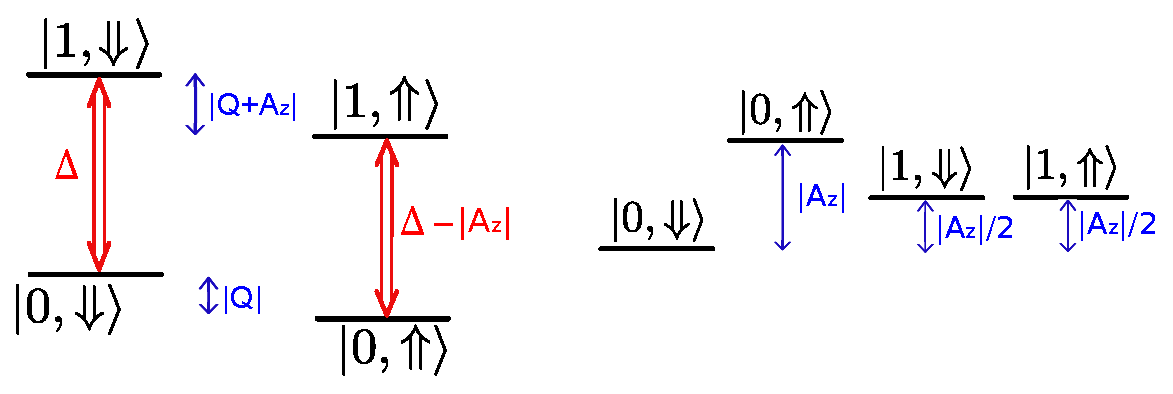
\includegraphics [width = 12 cm]{SOM/fig01_levelScheme.eps}
\caption{\textit{ On the left, scheme of the relevant energy levels for the electron and nuclear spin qubits. On the right, level energies in a doubly-rotating reference frame, rotating at frequency $\omega_e = \Delta-|A_z|/2$ for the electron spin, and $\omega_n = |Q+A_z|$ for the nuclear spin.}}
\label{fig:levels}
\end{figure} 


The Hamiltonian of the system is $\mathcal{\hat{H}}=\mathcal{\hat{H}}_0 +\mathcal{\hat{H}}_{drive}$, with:
\begin{equation}
 \mathcal{\hat{H}}_0 = -|Q| \dm{0, \Uparrow} + \Delta \dm{1, \Downarrow}+(\Delta-|Q+A_z|)\dm{1, \Uparrow}
\end{equation}
and:
\begin{equation}
 \mathcal{\hat{H}}_{drive} = \Omega_{MW} (t)  \hat{S}_{x} \otimes \mathbb{\hat{1}}_N  + \Omega_{RF} (t) \ket{1}\bra{1} \otimes \hat{I}_x + \mbox{h. c.}
 \label{Eq:ham0}
\end{equation}
where $\Delta= D -g_e \mu_eB = 2.8288 \pm 0.0002$  GHz and $\hat{S}_i$, $\hat{I}_i$ are respectively the Pauli operators for the electron spin and the nuclear spin. \\

The Hamiltonian in Eq. \ref{Eq:ham0} is time-dependent and state evolution has, in general, no analytical solution. In order to simplify the problem, we apply the rotating-wave approximation \cite{Slichter__1996}, using a doubly-rotating frame: one rotating at the driving frequency for the electron spin, and the other one at the driving frequency for the nuclear spin. We set the microwave  frequency ($\omega_e = \Delta-|A_z|/2$) such that it is detuned by $|A_z|/2$ from both hyperfine transitions and the RF-field is on resonance with the nuclear spin transition in the $m_s=-1$ electron spin manifold ($\omega_N = |Q+A_z|$). Applying the unitary transformation $\hat{U} = e^{-i \left( \omega_N \mathbb{\hat{1}}_e \times \hat{I}_z + \omega_e \hat{S}_z \times \mathbb{\hat{1}}_N \right) t}$ and retaining the secular terms, the Hamiltonian, in the basis $\{ \ket{0, \Downarrow}, \ket{0, \Uparrow}, \ket{1, \Downarrow}, \ket{1, \Uparrow}  \}$, becomes:

\begin{equation}
\mathcal{\hat{H}'} = \left[
\begin{array}{cccc}
0 & 0 & \Omega^*_{MW} & 0\\
0 & |A_z| & 0 & \Omega^*_{MW}\\
\Omega_{MW} & 0 & |A_z|/2 & \Omega^*_{RF}\\
0 & \Omega_{MW} & \Omega_{RF} & |A_z|/2
\end{array}
\right]
\label{eq:H0_RWA}
\end{equation}

The energy levels, in the rotating-wave approximation, are shown on the right side of Fig. \ref{fig:levels}. We define the positive quantity $A$ to be $A = |A_z|$ in the rest of the Supplementary Information.

\section{Qubit initialization}
The electron spin is initialized in the $m_s=0$ state by optical spin-pumping with a fidelity $0.983 \pm 0.006$ \cite{Robledo_Nature_2011}. We use the forbidden transition of $E_{y}$ which is detuned by $\Delta$ from the spin-preserving $E_{y}$-transition. This transition is well suited for a reset of the electron spin during the protocol, since flip-flops with the nuclear spin are suppressed due to selection rules. \\

\begin{figure} [h]
\centering
\includegraphics [width = 12 cm]{SOM/fig02_nuclearSpin_v2.eps}
\caption{\textit{On the left, nuclear spin initialization. The nuclear spin is initially unpolarized (gray): the ESR spectrum for the $m_s=-1 \leftrightarrow 0$ transition shows three hyperfine lines, corresponding to $m_I=-1,0,+1$. By measurement-based initialization (MBI) \cite{Pfaff_NatPhys_2012} we can initialize the spin in any of the nuclear spin states (blue/red). On the right, nuclear spin Ramsey. The nuclear spin is initialized by MBI after which the free evolution time $\tau$ between two $\pi/2$-pulses is varied. The solid line is a fit to the function $y_0 + e^{-(\frac{\tau}{T_{2}^{*}})^2}\cos{(\omega_{det} \tau + \phi )}$ from which we find the dephasing time $T_2^* = 7.8 \pm 0.2$ ms.}}
\label{fig:nuclearSpin}
\end{figure} 

The nuclear spin is initialized by measurement \cite{Pfaff_NatPhys_2012} as shown in Fig. \ref{fig:nuclearSpin}. We prepare the electron spin state in $\left| m_s=\pm 1 \right \rangle$ by spin-pumping on the $E_{y}$ transition. We apply a selective microwave $\pi$-pulse ($f_{rabi} = 181.8$ kHz) to the electron, on resonance with one of the three hyperfine lines. We then read-out the electron spin state, by exciting the $E_y$ transition. In case of photon detection, the electron state is projected to $m_s=0$, and the nuclear spin is projected on the state that was addressed by the microwave pulse.
During the selective microwave pulse, the electron spin undergoes significant dephasing, reducing the success probability, but not the initialization fidelity of the nuclear spin. The measured initialization fidelity is $0.95 \pm 0.02$, obtained from the fitting the heigth of the peaks in Fig. \ref{fig:nuclearSpin}  and the success probability is around $0.07$. The success probability is determined by $p = p_{m_s=-1} \cdot p_{m_I=-1} \cdot p_{e-flip} \cdot p_{phot}$, where the relevant parameters are:
\begin{itemize}
 \item $p_{m_s=-1} \sim 0.5$ is the probability to spin pump the electron spin in $m_s=-1$ (in the remaining cases it's in $m_s = +1$).
 \item $p_{m_I=-1} \sim 1/3$ is the population of the desired state $m_I=-1$ for an initially unpolarized nuclear spin.
 \item $p_{e-flip} \sim 0.6$ is the success probability of nuclear-dependent electron spin rotations.
 \item $ p_{phot} \sim 0.6-0.8$ is the probability to detect a photon when reading-out the $m_s=0$ state, limited by the collection of the optical system and the finite photon detection efficiency.
\end{itemize}


\section {Nucleus-independent electron spin rotations}

The maximum Rabi frequency we achieve in the setup is $\sim 8$ MHz (Fig. \ref{fig:rabi}). Given the hyperfine splitting of 2.184 MHz, these pulses introduce off-resonant driving errors that limit the weakest measurement we could achieve to $\theta = 15$ degrees ($C = 0.27$, see equation \ref{eq:concurrence}). To overcome this problem, we use CORPSE pulses \cite{Cummins_PRA_2003}, a composite pulse sequence designed to compensate for off-resonance errors. The weakest measurement we achieve with the CORPSE pulses is $\theta_{min} = 5$ degrees, corresponding to $\tau = 12$ ns (obtained from a fit of the Ramsey fringes in Fig. \ref{fig:amc-fig1}b of the main text)

\begin{figure} 
\centering
\includegraphics [width = 12 cm]{SOM/rabi.eps}
\caption{\textit{Coherent single-qubit rotations of the electron spin ancilla qubit (orange) and the nuclear spin system qubit (purple) are performed by varying the length of a MW (RF) pulse. Solid lines are sinusoidal fits from which we determine the Rabi frequency  $7.67 \pm 0.02$ MHz / $17.07 \pm 0.01$ kHz).}}
\label{fig:rabi}
\end{figure} 

\section{Electron-independent nuclear spin rotation}
\label {sec:uncond_rot_RF}
For quantum state tomography and for weak-value measurements, we need to be able to perform nuclear spin rotations, unconditional on the electron spin state. This is not trivial if the electron and nuclear spins are entangled.
In particular, when the electron is in the $\left| m_s=-1 \right \rangle$ state, the splitting between $\left| \Downarrow \right \rangle$ and $\left| \Uparrow \right \rangle$ is $\omega_N^{(-1)} = |Q+A_z| = 2\pi \times 7.164$ MHz, while when the electron in the $\left| m_s=0 \right \rangle$ state, $\omega_N^{(0)} = |Q| = 2\pi \times 4.98$ MHz. Given that the Rabi frequency of the nuclear spin is much smaller than the hyperfine interaction, the simple use of a hard $\pi$-pulse, as done for the electron, does not work. \\
We implemented the unconditional nuclear spin rotation using the scheme depicted in Fig. \ref{fig:RF}a. First we apply an RF pulse (RF-1) at $\omega_N^{(-1)}$, to rotate the nuclear spin when the electron spin is in the $\left| m_s=-1 \right \rangle$ manifold. We then apply a hard $\pi$-pulse to the electron and apply a second RF pulse (RF-2) at the same frequency $\omega_N^{(-1)}$.\\
As explained in Section \ref{sec:theory} (Eq. \ref{eq:state}), the partial measurement introduces a phase shift to the system qubit that depends on the measurement strength. The phase shift is proportional to the interaction time $\tau$ of the measurement. In order to characterize the phase shift, we used the following protocol:
\begin{itemize}
 \item we set the pulse length of RF-1 and RF-2 corresponding to a $\pi/2$ pulse ($T_{RF-1/2} = 14.6 \mu$s)
 \item we only apply the RF-1 pulse and sweep the phase of RF-1 for different values of $\tau$. Fitting the resulting sinusoidal signal, we recover the phase offset $\varphi_0^{(RF-1)} (\tau)$
 \item we then set the amplitude of RF-2 to the value corresponding to a $\pi/2$-pulse and without RF-1 apply a $\pi$-pulse on the electron followed by RF-2. We then sweep the phase of RF-2 for different values of $\tau$ and fit the sinusoid to reconstruct the phase offset $\varphi_0^{(RF-2)} (\tau)$
\end{itemize}
The values of the phase offsets as a function of $\tau$ for RF-1 and RF-2 ($\varphi_0^{(RF-1)} (\tau)$ and $\varphi_0^{(RF-1)} (\tau)$) are plotted in Fig. \ref{fig:RF}b. These values can be used to make sure that the resulting entangled nuclear-electron state has the correct phase when performing quantum state tomography (projections along $x$ and $y$ with a $\pi/2$-pulse along the corresponding axis and projection along $z$).\\
Furthermore, care should be taken that in general, while applying the first RF pulse (which rotates the nuclear spin by an angle $\Phi$ conditioned on the electron being in $\left| m_s=-1 \right \rangle$), the nuclear spin in the electron $ m_s=0$ manifold will undergo free-evolution, acquiring an additional phase shift proportional to the temporal length of the pulse (therefore to $\Phi$). Therefore, we need to characterize this phase offset for all situations different from a $\pi/2$-pulse. This was done by fixing $\tau$ and sweeping the phase of RF-2 for different value of the length of the RF-1 pulse ($T_{RF-1}$). After fitting the resulting sinusoidal oscillation, we retrieved the extra phase offset $\varphi_2 (\Phi)$ to RF-2 such that it is applied in the correct rotating frame. 

\begin{figure} [h]
\includegraphics [width = 12 cm]{SOM/fig03_RFpulses_v2.eps}
\caption{\textit {On the left, pulse sequence for unconditional nuclear spin rotation. On the right, phase of the nuclear spin as a function of the free evolution time $\tau$, for the two electron-spin manifolds ($m_S=-1$ and $m_S=0$).}}
\label{fig:RF}
\end{figure} 



\section{Partial measurements with controlled strength: Theory}
\label{sec:theory}
The protocol starts by initializing the nucleus in $\ket{\psi_N} = \frac{1}{\sqrt{2}} \left( \ket{\Downarrow}+\ket{\Uparrow} \right)$ and the electron in $\ket{\psi_e} = \ket{0}$.\\
The tunable-entangling gate consists of three steps. First, a $\pi/2$-pulse is applied around $x$ to the electron spin, creating the equal superposition state:
\begin{equation}
\left| \psi \right \rangle = \frac{1}{2} \left( \left| 0 \right \rangle - i \left| 1 \right \rangle \right) \left( \left| \Downarrow \right \rangle +\left| \Uparrow \right \rangle\right)
\end{equation}
Then the system undergoes free evolution of a variable time $\tau$ (according to the Hamiltonian in Eq. \ref{eq:H0_RWA}):
\begin{equation}
\ket{ \psi} = \frac{1}{2} \left \lbrace e^{0i} \ket{ 0, \Downarrow } + e^{-i A \tau} \ket{ 0, \Uparrow } - i  e^{-i A \tau/2} \ket{ 1, \Downarrow } - i  e^{-i A \tau/2} \ket{ 1, \Uparrow} \right \rbrace
\end{equation}
A second electron $\pi/2$-pulse, now around $y$, creates the state:
\begin{equation}
\left| \psi \right \rangle = \frac{1}{2} \left\lbrace \left| 0 \right \rangle \left[ \beta_+ (\tau) \left| \Downarrow \right \rangle + i e^{i A\tau/4} \beta_-(\tau) \left| \Uparrow \right \rangle \right] + e^{i\pi /2} \left| 1 \right \rangle \left[ \beta_-(\tau) \left| \Downarrow \right \rangle + i e^{i A\tau/4} \beta_+(\tau) \left| \Uparrow \right \rangle \right] \right\rbrace
\label{eq:state}
\end{equation}
where $\beta_{\pm} = \cos(\pi/4 \pm  A \tau/4)$. We define $\theta$ as $\theta= A \tau/2$, and the measurement strength as $\sin\theta$.\\
For $\theta=0$ ($\tau = 0$), the electron and nuclear spins are in a separable state:
\begin{equation}
\left| \psi (\tau=0) \right \rangle = \frac{1}{2} \left( \left| 0 \right \rangle +i \left| 1 \right \rangle \right) \left[ \left| \Downarrow \right \rangle +  i \left| \Uparrow \right \rangle \right]
\end{equation}
and a measurement of the electron spin gives no information about the state of the nuclear spin.
On the other hand, for $\theta = 90$ degrees (corresponding to $\tau = \pi/A = 229$ ns), the electron and nuclear spins are in a maximally-entangled state:
\begin{equation}
\left| \psi (\tau=\pi/A) \right \rangle = \frac{1}{\sqrt{2}} \left[ \left| 0, \Uparrow \right \rangle -i \left| 1, \Downarrow \right \rangle \right]
\end{equation}
and a measurement of the electron spin results in a projective measurement of the nuclear spin. Performing the electron-spin read-out by resonantly exciting the $E_y$ optical transition (therefore probing the population of the $\left| m_s=0 \right \rangle$ state) we project the nuclear spin on the $\left| m_I = -1 \right \rangle$ ($\ket{\Uparrow}$) state when a photon is detected and on the $\left| m_I = 0 \right \rangle$ ($\ket{\Downarrow}$) state when no photon is detected.\\
In the intermediate cases, $0<\tau<\pi/A$, the concurrence of the state as a function of $\tau$ is given by:
\begin{equation}
 C (\tau) = \sin\theta=\sin \left( A \tau/2 \right) 
\label{eq:concurrence}
\end{equation}
if $\ket{\psi_N}$ is initialized in $\ket{x}$. The value of C corresponds to the strength of the measurement performed on the system qubit.\\
Note from Eq. \ref{eq:state} that a $\tau$-dependent phase shift $\varphi = + A \tau/4$, unconditional on the electron spin, is imposed on the nuclear spin state after the measurement, as a result of the variable free evolution time. We compensate by adjusting the phase of the final RF pulse (see Section \ref{sec:uncond_rot_RF} for details).\\
The nuclear spin density matrix, unconditioned on the result of the electron spin measurement, can be derived by tracing over the electron spin, resulting in:
\begin{equation}
 \rho_{uncond} = \frac{1}{2}
 \left[
% \begin{center}
\begin{array}{cc}
1 & \cos^2 ( A \tau/2)\\
\cos^2 ( A \tau/2) & 1
 \end{array}
% \end{center}
 \right]
\label{eq:uncondRho}
 \end{equation}
Increasing the measurement strength, the initial pure state becomes increasingly mixed, resulting in a completely mixed state for $\theta = 90$ degrees.\\
 Conditioning on measuring the electron spin in the state $\ket{0}$, the nuclear spin state is:
\begin{equation}
 \rho_0 = \frac{1}{2}
 \left[
% \begin{center}
\begin{array}{cc}
1+\sin ( A \tau/2) & \cos^2 ( A \tau/2)\\
\cos^2 ( A \tau/2) & 1-\sin(A \tau/2)
 \end{array}
% \end{center}
 \right]
 \label{eq:condRho}
\end{equation}
Now, the resulting state remains pure, but it is increasingly rotated towards $\ket{\Uparrow}$ for increasing measurement strength. 

\section{Characterization of the partial measurements}
The partial measurement was characterized by performing quantum state tomography, as explained in the main text. In Fig \ref{fig:backaction}, we plot the elements of the density matrix of the nuclear spin after the partial measurement as a function of the measurement strength, for three different input states $\{ \ket{\Uparrow}, \ket{x}, \ket{y} \}$. On the upper row we do not take the measurement outcome of the electron into account, while on the lower row we show the data conditioned on the detection of a photon (ancilla projected to $\ket{0}$).\\
When we condition on a measurement result for the ancilla, the operation on the system qubit is a projection with increasing strength (completely projective along $z$ for measurement strength 1). In the unconditioned case, we observe measurement-induced dephasing.

\begin{figure} 
\includegraphics [width = 12 cm]{SOM/fig04_backAction.eps}
\caption{\textit{Density matrix elements of the states after a partial measurement, as a function of the measurement strength, for three different input states. On the upper row, data not taking the electron spin readout into account. On the lower row, data conditioned on detection of a photon (electron spin projected to $m_s = 0$). Solid lines represent theoretical prediction from Eq. \ref{eq:uncondRho} and Eq. \ref{eq:condRho}}}
\label{fig:backaction}
\end{figure} 


We characterized the collapse process by quantum process tomography \cite{Nielsen__2000}. Results are plotted in Fig. \ref{fig:QPT}. On the upper row, the process matrix for the unconditioned case shows a continuous transition from the identity process to a collapse process consisting of equal contributions of $\mathbb{\hat{1}}$ and $\hat{\sigma}_z$: the absence of off-diagonal terms represents the increasing dephasing. The theoretical process matrix for the unconditioned case is:
\begin{equation}
 \hat{\chi}_{uncond} = \frac{1}{2}
 \left[
\begin{array}{cccc}
1+\cos\theta & 0 & 0 & 0\\
0 & 0 & 0 & 0\\
0 & 0 & 0 & 0\\
0 & 0 & 0 & 1-\cos\theta
 \end{array}
 \right]
\end{equation}
On the bottom row, we plot the process conditioned on the measurement result of the electron spin: this is a non-trace-preserving process, with state-dependent success probability \cite{Bongioanni_Phys.Rev.A_2010}. The theoretical process matrix as a function of $\theta$ is:
\begin{equation}
\hat{\chi}_{cond} = \frac{1}{2}
 \left[
\begin{array}{cccc}
1+\cos\theta & 0 & 0 & \sin\theta\\
0 & 0 & 0 & 0\\
0 & 0 & 0 & 0\\
\sin\theta & 0 & 0 & 1-\cos\theta
 \end{array}
 \right]
\end{equation}
In this case, the process is coherent and the off-diagonal terms are, in general, non-zero. The fidelity between the ideal process matrix and our experimentally reconstructed one is plotted in Fig. \ref{fig:QPT_fid}.


\begin{figure} 
\centering
\includegraphics [width = 12 cm]{SOM/fig05_QPT.eps}
\caption{\textit{ Quantum process tomography for the tunable-strength measurement for different strength values (defined by the value of $\tau$ and the corresponding values for $\theta =  A \tau/2$ and measurement strength $C=\sin\theta$). On the upper row, the real part of the process matrix for the unconditioned case. On the lower row, the process matrix conditioned on a measurement of the ancilla giving the result $\ket{0}$.}}
\label{fig:QPT}
\end{figure} 


\begin{figure} 
\centering
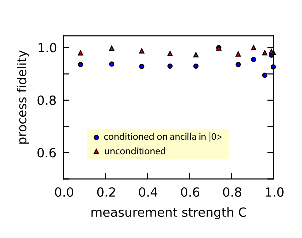
\includegraphics [width = 6 cm]{SOM/fig06_QPTfidelity.eps}
\caption{\textit{ Fidelity of the reconstructed quantum process matrices $\chi_{cond}$ and $\chi_{uncond}$, as a function of the measurement strength ($C = \sin\theta$). The fidelity is calculated with the formula: $F (\chi_{exp}, \chi_{th})  = \mbox{Tr} \left \lbrace \sqrt{\sqrt{\chi_{exp}} \chi_{th} \sqrt{\chi_{exp}}} \right\rbrace^2$ \cite{Bongioanni_Phys.Rev.A_2010}.}}
\label{fig:QPT_fid}
\end{figure} 

\section {Weak value and conditioned average}
Given an observable $\mathcal{I}$, the weak value of the associated quantum operator $\hat{I}$, as introduced by Aharonov, Albert and Vaidman \cite{Aharonov_PRL_1988,Kofman_PhysicsReports_2012}, is defined by

\begin{equation}
\label{eq:wv}
 I_W = \frac{ \bra{\psi_f} \hat{I} \ket{\psi_i}}{\left \langle \psi_f | \psi_i \right \rangle }
\end{equation}
This quantity does not depend on the context of the specific measurement, but only on the operator $\hat{A}$ and on the initial and final states (respectively $\left| \psi_i \right \rangle$ and $\left| \psi_f \right \rangle$). For a qubit, with initial state $\ket{\psi_i} = \ket{x}$ and final state $\ket{\psi_f}  = \cos \phi \ket{0} + \sin \phi \ket{1}$, we have $(S_z)_w = \cos 2\phi/(1+\sin 2\phi)$.\\
Given an observable $\mathcal{A}$, one can measure it with a series of operators, which can be projectors $\lbrace \hat{\Pi}_k , \hat{\Pi}_k^2 = \hat{\Pi}_k\rbrace$ or, more generally, POVMs $\lbrace \hat{E}_j = \hat{M}^{\dagger}_j \hat{M}_j \rbrace$. The associated measurement outcomes are, respectively, the eigenvalues $\left \lbrace a_k \right \rbrace$ and the generalized eigenvalues (or contextual values) $\left \lbrace \alpha_j \right \rbrace$ \cite{Dressel_Phys.Rev.Lett._2010}, such that the spectral decomposition of the operator $\hat{I}$ can be written as:
\begin{equation}
 \hat{I} = \sum_j \alpha_j \hat{E}_j = \sum_k a_k \hat{\Pi}_k
\end{equation}


Consider now a sequence of two measurements, $\mathcal{M}_1$ and $\mathcal{M}_2$ and suppose to condition the average of the result of  $\mathcal{M}_1$ to a measurement result for $\mathcal{M}_2$. The generalized weak value (or conditioned average) of the observable is defined as:
\begin{equation}
 _f \left \langle I \right \rangle = \sum_j \alpha_j^{(1)} P(j|f)
\end{equation}
where $\lbrace \alpha_j^{(1)}\rbrace$ are the possible measurement outcomes of $\mathcal{M}_1$ (generalized eigenvalues) and $P(j|f) = p_{jf}/(\sum_j p_{jf})$ is the conditional probability to detect the outcome $\alpha_j^{(1)}$ in the first measurement, given the outcome $\alpha_f^{(2)}$ for the second measurement.\\
Unlike the weak value, the conditioned average encodes information not only about the observable $\mathcal{A}$, but also on the specific measurement context. However, it can be shown \cite{Dressel_Phys.Rev.Lett._2010} that, under certain conditions (namely minimal state disturbance), the dependence on the measurement vanishes. For a pure initial state, a pure POVM and a projective final measurement, it reduces to the weak value of Eq. \ref{eq:wv} .\\
In our case, for a measurement operator $\hat{E}_j = (1/2) (\mathbb{\hat{1}} \pm \sin\theta \hat{I}_z)$, the generalized eigenvalues are $\pm 1/\sin\theta$ and the conditional average is:
\begin{equation}
\label{eq:cond_avg}
 _f \left \langle I_z \right \rangle = \frac{1}{\sin\theta} \frac{p_{00}-p_{10}}{p_{00}+p_{10}}  = \frac{\cos 2\phi}{1+ \cos \theta \sin 2\phi}
\end{equation}
This quantity reduces to the quantum weak value for $\sin\theta = 0$ and does not diverge for finite measurement strength. Note that from this expression \cite{Williams_PRL_2008,Groen_PRL_2013}, it is possible to observe values lying outside the range of the operator eigenvalues for any finite measurement strength.
\\

\section {Experimental quantum weak value for a spin qubit}
A measurement of the conditional average $ _f \left \langle I_z \right \rangle$ is performed with the pulse sequence shown in Fig. \ref{fig:amc-fig1}a of the main text, starting from the initial state $\ket{x} = (1/\sqrt{2}) \left( \ket{\Downarrow} + \ket{\Uparrow} \right)$. The scheme consists of a partial measurement (strength $\theta$) followed by a projective measurement in a rotated basis (angle $\phi$), post-selecting on the result of the projective measurement. In the first set of measurements (large panel in Fig. \ref{fig:amc-fig2}d of the main text) we fix the strength of the first measurement and sweep the basis rotation angle $\phi$ before the projective measurement. For the inset of Fig. \ref{fig:amc-fig2}d of the main text we sweep the measurement strength $\theta$ and choose $\phi$ to yield the maximum weak value. \\
We post-select on the measurement outcome $\ket{0}$ for the ancilla read-out (system in $\ket{\Uparrow}$), corresponding to the detection of a photon (electron spin in $m_s=0$). \\
The conditional average can be calculated with the expression in Eq. \ref {eq:cond_avg} where $p_{ij}$ is the probability of outcome $i$ for the ancilla read-out of the partial measurement and measurement outcome $j$ for the ancilla read-out of the projective measurement (assuming perfect readout). From Eq. \ref{eq:state}, we calculate the dependence of $p_{ij}$ on $\phi$ and $\theta$:
\begin{equation}
\label{eq:prob_wm}
  \begin{split}
  p_{11}&=\frac{1}{2} \left[ \beta_-(\theta) \cos\phi + \beta_+ (\theta) \sin\phi \right]^2  \\
  p_{10}&= \frac{1}{2} \left[ \beta_-(\theta) \sin\phi - \beta_+ (\theta) \cos\phi\right]^2 \\
  p_{01}&= \frac{1}{2} \left[ \beta_-(\theta) \sin\phi + \beta_+ (\theta) \cos\phi\right]^2 \\
  p_{00}&=\frac{1}{2} \left[ \beta_-(\theta) \cos\phi - \beta_+ (\theta) \sin\phi \right]^2 
  \end{split}
\end{equation}
where $\beta_{\pm} (\theta) = \cos (\pi/4 \pm \theta/2)$.\\
 
Since our read-out is not perfect, it must be calibrated to take into account the finite detection efficiency and the dark counts. For the state $m_s=0$ we are limited by our detection efficiency ($\sim .80$), while for the $m_s=-1$ read-out we suffer from dark counts. We define $F_i$ as the fidelity of the $m_s=0$ read-out and $G_i$ as the read-out fidelity for $m_s=-1$, in the $i-$th measurement.
Then, given the ideal probabilities $p_{ij}$, the measured fractions $n_{ij}$ are:
 
\begin{equation}
\resizebox{.9\hsize}{!}{$
\left[
\begin{array}{c}
n_{11}\\
n_{10}\\
n_{01}\\
n_{00}
 \end{array}
 \right]=
 \left[
\begin{array}{cccc}
G_1 G_2 & G_1(1-F_2) & (1-F_1)G_2 & (1-F_1)(1-F_2)\\
G_1(1-G_2) & G_1 F_2 & (1-F_1)(1-G_2) & F_2(1-F_1)\\
(1-G_1)G_2 & (1-G_1)(1-F_2) & F_1 G_2 & F_1(1-F_2)\\
(1-G_1)(1-G_2) & (1-G_1)F_2 & F_1 (1-G_2) & F_1 F_2
 \end{array}
 \right]
\left[
\begin{array}{c}
p_{11}\\
p_{10}\\
p_{01}\\
p_{00}
 \end{array}
 \right] $}
\label{ROcor}
\end{equation}
The theoretical curve in Fig. \ref{fig:amc-fig2}d of the main text is calculated without fit-parameters, using the read-out correction of Eq. \ref{ROcor} and assuming an asymmetric spin-flip rate $f= 0.02$ between the first and second read-out. This spin-flip probability arises during the reset of the ancilla by optically exciting the forbidden transition of Ey. The value $f$ is determined from independent measurements. \\


\section{Partial measurements as probabilistic rotations}
Starting from the state $\ket{\psi_{init}} =  \cos\theta_i \ket{\Downarrow}+ \sin\theta_i \ket{\Uparrow} $, we perform a partial measurement with strength $\theta_m$. With probability $\cos^2\theta$, we obtain the state:
\begin{equation}
 \ket{\psi_0} = \frac{1}{\mathcal{N}_0} \left[ \cos \left( \pi/4 + \theta_m/2 \right) \cos\theta_i \ket{\Downarrow} +  \cos \left( \pi/4 - \theta_m/2 \right) \sin\theta_i \ket{\Uparrow} \right]
\end{equation}
where $1/\mathcal{N}_0$ is the normalization factor. The state, initially at an angle $\theta_i$, is rotated to the angle:
\begin{equation}
 \theta_0 = \arctan{ \left[ \tan\theta_i \frac{\cos\theta_m}{1-\sin\theta_m} \right]}
\end{equation}
On the other hand, with probability $p_{succ} = \sin^2\theta$, the measurmeent leads to the state:
\begin{equation}
 \ket{\psi_1} = \frac{1}{\mathcal{N}_1} \left[ \cos \left( \pi/4 - \theta_m/2 \right) \cos\theta_i \ket{\Downarrow} +  \cos \left( \pi/4 + \theta_m/2 \right) \sin\theta_i \ket{\Uparrow} \right]
\end{equation}
Therefore, the initial state rotated to the angle:
\begin{equation}
 \theta_1 = \arctan{ \left[ \tan\theta_i \frac{1-\sin\theta_m}{\cos\theta_m} \right]}
\end{equation}
In other words, as shown in \cite{Jordan_PRB_2006}, a partial measurement is equivalent to a probabilistic state rotation, with a rotation angle which depends on the strength of the measurement and on the initial state (see Fig. \ref{fig:prob_rot}).

\begin{figure} 
\centering
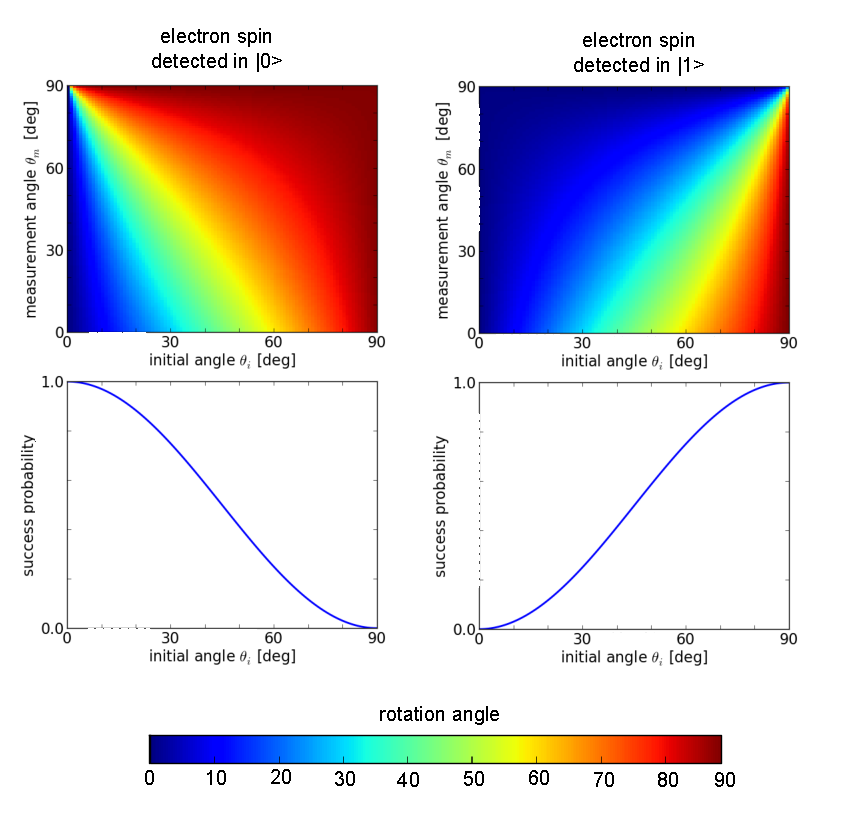
\includegraphics [width = 12 cm]{SOM/fig07_prob_rotation.eps}
\caption{\textit{A partial measurement is equivalent to a probabilistic rotation. Given a an initial superposition with angle $\theta_i$ ($\ket{\psi_{init}} =  \cos\theta_i \ket{\Downarrow}+ \sin\theta_i \ket{\Uparrow} $) and a partial measurement with strength $\theta_m$, one gets the rotation angle plotted on the upper left subplot in case the electron spin is measured to be in $\ket{0}$ (probability $\cos^2 \theta_i$, plot on the bottom left) or the rotation angle plotted on the upper right in case the electron spin is measured to be in $\ket{1}$ (probability $\sin^2 \theta_i$, plot on the bottom right)}}
\label{fig:prob_rot}
\end{figure} 


\section{Heralded sequential measurements: un-collapse and steering}
In Fig. \ref{fig:uncollapse}, we implement two heralded sequential partial measurements. We post-select on the case of photon detection, using short read-out times to minimize electron spin-flips, at the price of reduced success probabilities. We can do this with high fidelity, maintaining a good coherence of the state after two measurements. No spin-pumping between the two measurements is performed, in order to avoid electron spin-flips that would destroy nuclear-spin coherence.\\
We first perform a measurement with strength $\theta_1=20$ degrees, followed by a measurement with the same strength but projecting on the opposite electron state (equivalent to a measurement with strength $\theta_2=-20$ degrees). This brings us back to the original quantum state, in a probabilistic un-collapse of the state. This technique has been used to probabilistically recover a state subject to amplitude-damping decoherence \cite{Koashi_Phys.Rev.Lett._1999,Korotkov_Phys.Rev.Lett._2006,Katz_Phys.Rev.Lett._2008}.  \\
In general, a partial quantum measurement is equivalent to a probabilistic rotation. For $\theta_1=\theta_2=+20$ degrees, two successive measurements result in a combined rotation of $39$ degrees, with success probability $0.16$. In our case, heralding on photon detection, this can be done quite effectively (fidelity $0.78$).

\begin{figure} 
\centering
\includegraphics [width = 12 cm]{SOM/fig08_uncollapse.eps}
\caption{\textit{Two sequential heralded partial measurements, both post-selected on the case of photon detection. The density matrices are the result of state tomography, performed after the two partial measurements. For the uncollapse (upper density matrix), first a measurement with strength $C = 0.34$ ($\theta_1=20$ degrees) is performed, after which the initial state is restored by a second measurement with $\theta_2 = -20$ degrees. For the lower density matrix, the second measurement is set to  $\theta_2 = 39$ degrees, such that the system, that was projected towards $|\downarrow >$ after the first measurements,  is steered towards $|\uparrow >$ through the backaction of the second measurement.}}
\label{fig:uncollapse}
\end{figure} 

\section{State steering by real-time adaptive measurements}
\subsection{Ideal protocol}
We start in the state $\left| \psi_0 \right \rangle = \ket{x} = (1/\sqrt{2}) \left(\left| \Downarrow \right \rangle + \left| \Uparrow \right \rangle \right)$, with the goal to reach a target state $\left| \psi_T \right \rangle = \cos\theta_T \left| \Downarrow \right \rangle + \sin\theta_T \left| \Uparrow \right \rangle$.\\
First, we do a measurement with strength $\theta_1 = \pi/2-2\theta_T$. With probability $0.5$ the system reaches the target state, while in the rest of the cases it is shifted in the oppposite direction, to the state:
\begin{equation}
\left| \psi_1 \right \rangle = \cos \left( \frac{\pi}{4} - \frac{\theta_1}{2} \right) \left| \Downarrow \right \rangle + \cos \left( \frac{\pi}{4} + \frac{\theta_1}{2} \right) \left| \Uparrow \right \rangle
\end{equation}
In order to try to steer it back, we perform a second measurement, with strength $\theta_2$. In case of success, we get the state:
\begin{equation}
\resizebox{.9\hsize}{!}{$
\left| \psi_{10} \right \rangle = \frac{1}{\mathcal{N}} \left[ \cos \left( \frac{\pi}{4} - \frac{\theta_1}{2} \right)\cos \left( \frac{\pi}{4} + \frac{\theta_2}{2} \right) \left| \Downarrow \right \rangle + \cos \left( \frac{\pi}{4} + \frac{\theta_1}{2} \right)\cos \left( \frac{\pi}{4} - \frac{\theta_2}{2} \right) \left| \Uparrow \right \rangle \right]
$}
\end{equation}
where $\mathcal{N} = \left[ \cos^{2} \left( \frac{\pi}{4} - \frac{\theta_1}{2} \right)\cos^2 \left( \frac{\pi}{4} + \frac{\theta_2}{2} \right) + \cos^2 \left( \frac{\pi}{4} + \frac{\theta_1}{2} \right) \cos^2 \left( \frac{\pi}{4} - \frac{\theta_2}{2} \right) \right]^{1/2}$.
The system can be steered to target state, by setting:
\begin{equation}
 \frac{1}{\mathcal{N}} \cos \left( \frac{\pi}{4} - \frac{\theta_1}{2} \right)\cos \left( \frac{\pi}{4} + \frac{\theta_2}{2} \right) = \cos \left( \frac{\pi}{4} + \frac{\theta_1}{2} \right)
\end{equation}
After simplification, this leads to the equation:
\begin{equation}
\left( 1 + \sin \theta_1 \right) \left( 1 - \sin \theta_2 \right) = \left( 1 - \sin \theta_1 \right) \left( 1 - \sin \theta_1 \sin \theta_2 \right)
\end{equation}
Solving for $\theta_2$, we find that the strength of the second measurement can be tuned as:
\begin{equation}
 \theta_2 =  \sin^{-1} \left[ 2\frac{\sin \theta_1}{1+\sin^2 \theta_1} \right]
\end{equation}
The probability to steer the state to the desired target, after two measurements, is:
\begin{equation}
 p_{success} = \frac{ 1 + \cos \theta_1 }{2}
\end{equation}


\begin{figure} 
\centering
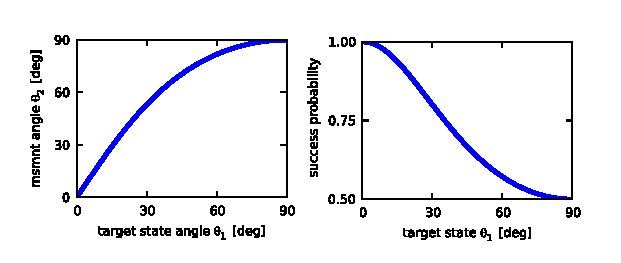
\includegraphics [width = 12 cm]{SOM/fig09_adaptMsmsnt_angle.eps}
\caption{\textit{On the left, strength of the second measurement, as a function of the desired target state. On the right, success probability of the two-step algorithm.}}
\label{}
\end{figure} 


\subsection{Error analysis}
The protocol described in the last Section assumes ideal measurements. In practice, however, we are subject to several non-ideal conditions \cite{Robledo_Nature_2011}:
\begin{itemize}
 \item the electron-spin read-out is not perfect. Given that the electron is in $m_s=0$, if we excite the $E_{y}$ transition, we are supposed to detect photons. However, such photons are detected with a finite efficiency (due to losses in the diamond, the collection optics and the finite efficiency of the detector). This results in a read-out fidelity $F_0 < 1$. In the first measurement, this leads us to make the wrong decision and apply a correction although we had already reached the target state.
 \item due to dark counts, we detect photon clicks even in the absence of photons. This probability is quite small, so we neglect it in the following analysis
 \item during electron read-out, there is a probability ($q$) that the electron spin flips. This results in dephasing of the nuclear spin. Moreover, with a small probability it results also in a nuclear spin-flip (we measured the probability to get a nuclear spin-flip as a result of an electron spin-flip to be around $0.02$). We neglect the nuclear spin flip and just consider the effect of dephasing.
\end{itemize}

The read-out efficiency and spin-flip probability are not independent: the longer the read-out, the higher the detection efficiency, but, at the same time, the electron spin-flip probability is also increased. The read-out fidelity $F_0$ and the electron spin-flip probability $q$, as a function of read-out time, are shown in the inset of Fig. \ref{fig:adaptiveScheme}. The best trade-off is for a read-out time $T \sim 5 \mu$s, where $F_0 \sim 0.6$ and $q \sim 0.2$.

\begin{figure} 
\centering
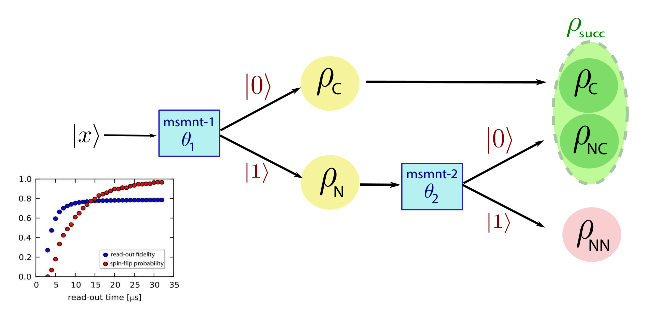
\includegraphics [width = 12 cm]{SOM/fig10_adaptiveScheme.eps}
\caption{\textit{Description of the adaptive scheme. Ancilla readout $\ket{0}$ corresponds to the detection of a photon when optically exciting the $E_{y}$ transition, while no photon detection corresponds to ancilla projection to $\ket{1}$. Inset: experimental data for electron spin read-out fidelity $F_0$ and spin-flip probability $q$ as a function of read-out time.}}
\label{fig:adaptiveScheme}
\end{figure} 

We prepare the initial $\ket{x}$ state and perform the first measurement. With probability $p_C = 0.5 F_0$, the ancilla readout outcome is $\ket{0}$ (corresponding to a photon detection event) and we take the upper branch of Fig. \ref{fig:adaptiveScheme}. The resulting density matrix is:
\begin{equation}
\begin{split}
 \rho_C &= (1-q) \ket{\psi_0}\bra{\psi_0} + q \rho_0^{(deph)}\\
 &= \frac{1}{2} \left[
\begin{array}{cc}
1-\sin\theta_1 & (1-q) \cos\theta_1\\
(1-q) \cos\theta_1 & 1+\sin \theta_1
\end{array}
\right]
\end{split}
\end{equation}

The density matrix $\rho^{(deph)}$ is the completely-mixed equivalent of the density matrix $\rho$, with zero off-diagonal elements. 
For no electron spin-flips ($q = 0$) this would just be the density matrix of the pure target state.
On the other hand, for perfect ancilla readout fidelity ($F_0=1$), the measurement outcome $\ket{1}$ would lead to the following density matrix (in the lower branch of Fig. \ref{fig:adaptiveScheme}):
\begin{equation}
\begin{split}
 \rho_W &= (1-q) \ket{\psi_1}\bra{\psi_1} + q \rho_1^{(deph)}\\
&=
\frac{1}{2}
\left[
\begin{array}{cc}
1+\sin\theta_1 & (1-q) \cos\theta_1\\
(1-q) \cos\theta_1 & 1-\sin \theta_1
\end{array}
\right]
\end{split}
\end{equation}

However, we get into the lower branch of Fig. \ref{fig:adaptiveScheme} also when we are supposed to get the outcome $\ket{0}$ but, due to the imperfect read-out (fidelity $F_0<1$), we missed the corresponding photon, which lead us to believe that the measurement outcome was $\ket{1}$. Taking this into account, the density matrix results for ancilla measurement outcome $\ket{1}$ is composed by two terms:
\begin{equation}
 \rho_N \sim 0.5 \rho_W + 0.5 (1-F_0) \rho_C
 \label{eq:rhoN}
\end{equation}
The total probability to be in the lower branch of Fig. \ref{fig:adaptiveScheme} is $p_W = 1- 0.5 F_0$.\\
If we are in the lower branch, we try to reach the target state by performing a second measurement, which is successful (ancilla projected to $\ket{0}$) with probability $p_1 (\theta_1)$. In this case, the component $\rho_W$ is rotated back to the target state, with some spin-flip probability and the corresponding dephasing:
\begin{equation}
 \rho_{W}' = (1-q) \left[ (1-q) \ket{\psi_0}\bra{\psi_0} + q \rho_0^{(deph)} \right] +q \rho_1^{(deph)}
\end{equation}
The component $\rho_C$ is, on the other end, rotated in the wrong direction:
\begin{equation}
  \rho_{C}' = (1-q) \left[ (1-q) \ket{\psi_2}\bra{\psi_2} + q \rho_2^{(deph)} \right] +q \rho_0^{(deph)}
 \label{eq:rho1c}
\end{equation}

The density matrix, for ancilla measurement outcome $\ket{1}$ in the second measurement is:
\begin{equation}
 \rho_{NC} = \frac{1}{1-0.5F_0} \left[ 0.5 \rho_W' + 0.5 (1-F_0) \rho_C' \right]
\end{equation}
%where $\rho_{deph} = q \left[ \rho_0^{(deph)} +(1-F_0) \rho_2^{(deph)} \right] +q \rho_1^{(deph)}$.
It consists of three terms: a contribution $\ket{\psi_0}\bra{\psi_0}$ which has been correctly recovered by the adaptive measurement, an error contribution $\ket{\psi_2}\bra{\psi_2}$ (due to wrong feedback) and a dephased contribution (due to imperfect read-out).\\
The density matrix $\rho_{succ}$, taking into account the cases where our protocol heralds success (so either detecting a photon in the first measurement, or only detecting a photon in the second measurement) is:
\begin{equation}
\rho_{succ} = \frac{1}{p_1 + 0.5 F_0} \left[  0.5 F_0  \rho_C + p_1 \rho_{NC} \right]
\end{equation}


The state fidelity is then calculated as $\mathcal{F} = \bra{\psi_0} \rho_{succ} \ket{\psi_0}$.
\begin{figure} [h]
\centering
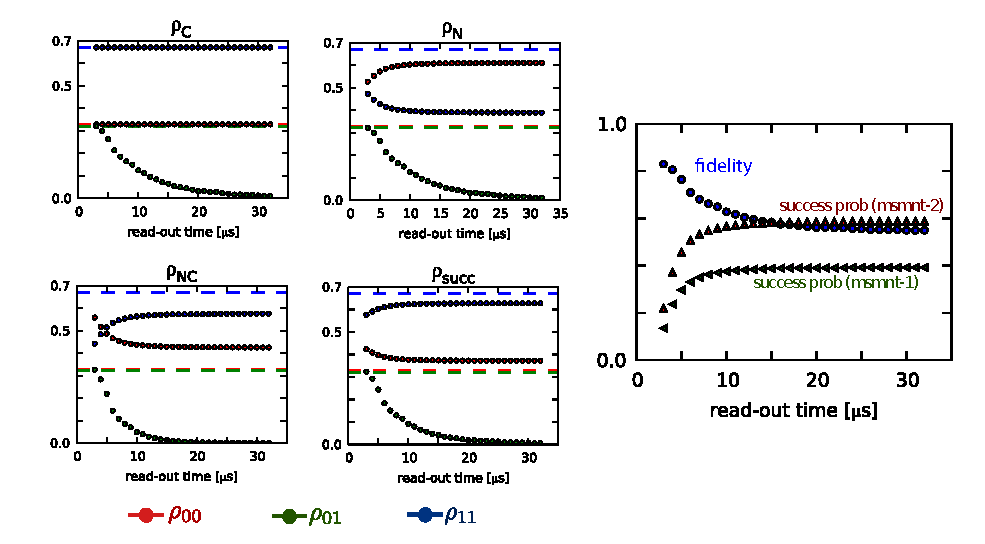
\includegraphics [width = 12 cm]{SOM/fig11_adaptiveScheme_normalRO.eps}
\caption{\textit{Realistic model for the adaptive scheme. On the left, density matrix elements for the different states in Fig. \ref{fig:adaptiveScheme}. On the right, success probabilities and state fidelity as a function of electron spin read-out time.}}
\label{fig:sim_adapt_fullRO}
\end{figure} 
The results of the simulation are plotted in Fig. \ref{fig:sim_adapt_fullRO}. For each of the four plots on the left, we show the three elements of the density matrix ($\rho_{00}$, $\rho_{01}$ and $\rho_{11}$). \\

For measurement outcome $\ket{0}$ in the ancilla readout in the first measurement, we take the upper branch in the scheme in Fig. \ref{fig:adaptiveScheme}, resulting in the density matrix $\rho_C$. This density matrix shows correct values for the $z$-components, independently of the read-out time. Increasing the read-out time, we increase the probability of taking the upper branch, up to a maximum value $0.5 \times 0.8 = 0.4$, in the case $F_0=0.8$. However, the dephasing also increases, together with the success probability, as shown on the right plot (green curve, success probability measurement-1). \\
For measurement outcome $\ket{1}$, we take the lower branch and get the state described by the density matrix $\rho_N$. The elements of $\rho_N$ (Eq. \ref{eq:rhoN}) are, as expected, the opposite of the target state: for longer read-out time, however, they do not saturate to the exact opposite value, since there is also a component of state that would be the correct one, but is in the wrong branch because the associated photons were not detected.\\
Considering the second measurement, ancilla measurement outcome $\ket{0}$ leads us to $\rho_{NC}$. In this case, we manage to invert the matrix elements and restore a density matrix more similar to the target one, but not completely because the restoring transformation has been also applied to the correct component, making it wrong (state described by $\rho_C'$ in Eq. \ref{eq:rho1c}). \\
Combining $\rho_C$ and $\rho_{NC}$, we get $\rho_{succ}$. Two features are important: the longer the read-out time, the higher read-out fidelity and therefore the more frequently the right choice is made in the adaptive step. This reflects in a higher fidelity of the $z$ components of the density matrix and higher success probability (red curve on the right plot). On the other hand, for longer read-out time, the probability of ancilla spin-flips is higher, which results in increasing dephasing. In the right plot, this is clear from the trade-off between state fidelity and success probability.

\begin{figure} 
\centering
\includegraphics [width = 12 cm]{SOM/fig12_results_normalRO.eps}
\caption{\textit{Experimental results for success probability (on the left) and state fidelity (on the right) for the adaptive measurement protocol, using full electron-spin read-out}}
\label{fig:exp_adapt_fullRO}
\end{figure} 

In Fig. \ref{fig:exp_adapt_fullRO}, we plot the experimental results obtained using full electron-spin read-out. Compared to the results reported in the main text (Fig. 4, dynamical-stop read-out), the state is completely dephased after about $20 \mu$s and the fidelity decreases quickly to around $0.6$.

\subsection{Dynamical-stop electron read-out}


As described in the main text, dynamical-stop electron spin read-out allows us to reduce the dephasing on the nuclear spin induced by electron measurement. To model the effect of dynamical-stop read-out we take the assumption that read-out stops as soon as a photon is detected, causing no electron spin-flip and no nuclear-spin dephasing. The assumption of no nuclear-spin dephasing is not confirmed by experimental data in Fig. 3c of the main text: however, it is justified to use it here for a simple model that gives a higher bound on the expected fidelity. \\

The results of the model for dynamical-stop read-out are reported in Fig. \ref{fig:model_segmRO}. Compared to Fig. \ref{fig:sim_adapt_fullRO}, the state $\rho_C$ is not dephased, while $\rho_N$ is similar to the one for full read-out. This results, in a much less dephased state in case of success ($\rho_{succ}$). The fidelities for the case when using full electron-spin read-out or dynamical-stop read-out are plotted on the right side of Fig. \ref{fig:model_segmRO}.
\begin{figure} [h]
\centering
\includegraphics [width = 12 cm]{SOM/fig13_adaptiveSceheme_dynStopRO.eps}
\caption{\textit{Model of the adaptive scheme results, using dynamical read-out. On the left, density matrix elements for the states at different stages of the protocol on Fig. \ref{fig:adaptiveScheme}. On the right, comparison between state fidelity using conventional electron read-out and dynamical-stop read-out.}}
\label{fig:model_segmRO}
\end{figure} 


\newpage
\bibliographystyle{../thesis}
\bibliography{amc_appendix}
